\documentclass{beamer}
%
% Choose how your presentation looks.
%
% For more themes, color themes and font themes, see:
% http://deic.uab.es/~iblanes/beamer_gallery/index_by_theme.html
%

\usefonttheme{professionalfonts}
\usefonttheme{serif}
\usepackage{fontspec}
\setmainfont{Helvetica Neue}
\setbeamerfont{note page}{family*=pplx,size=\footnotesize} % Palatino for notes

\usepackage{listings}
\lstset{
  frame=top|bottom,
  basicstyle=\tiny,    % the size of the fonts that are used for the code
  tabsize=2,                              % tab size in blank spaces
  extendedchars=true,                     %
  breaklines=true,                        % sets automatic line breaking
  captionpos=b,                           % sets the caption-position to top
  mathescape=true,
  showspaces=false,           % Leerzeichen anzeigen ?
  showtabs=false,             % Tabs anzeigen ?
  xleftmargin=17pt,
  belowcaptionskip=1em,
  aboveskip=2em,
  framexleftmargin=17pt,
  framexrightmargin=17pt,
  framexbottommargin=5pt,
  framextopmargin=5pt,
  showstringspaces=false      % Leerzeichen in Strings anzeigen ?
 }

\setbeamertemplate{frametitle}
{
   \begin{centering}
   \smallskip
   \huge\insertframetitle\smallskip\par
   \usebeamercolor[fg]{framesubtitle}\footnotesize\textit{\insertframesubtitle}\par
   \smallskip
   \end{centering}
}
\setbeamertemplate{itemize item}{--}
\setbeameroption{show notes}
\setbeamertemplate{navigation symbols}{}
\setbeamertemplate{footline}{%
    \raisebox{5pt}{\makebox[\paperwidth]{\hfill\makebox[20pt]{\color{gray}
          \scriptsize\insertframenumber}}}\hspace*{5pt}
}

\definecolor{foreground}{HTML}{D7D0CE}
\definecolor{background}{RGB}{24,24,24}
\definecolor{title}{HTML}{2380FC}
\definecolor{gray}{RGB}{155,155,155}
\definecolor{subtitle}{RGB}{102,255,204}
\definecolor{hilight}{RGB}{102,255,204}
\definecolor{vhilight}{RGB}{255,111,207}
\definecolor{alert}{HTML}{FC4438}

\setbeamercolor{titlelike}{fg=title}
\setbeamercolor{subtitle}{fg=subtitle}
\setbeamercolor{framesubtitle}{fg=subtitle}
\setbeamercolor{institute}{fg=gray}
\setbeamercolor{normal text}{fg=foreground,bg=background}
\setbeamercolor{item}{fg=foreground} % color of bullets
\setbeamercolor{subitem}{fg=gray}
\setbeamercolor{alerted text}{fg=alert}
\setbeamercolor{itemize/enumerate subbody}{fg=gray}
\setbeamertemplate{itemize subitem}{{\textendash}}
\setbeamerfont{itemize/enumerate subbody}{size=\footnotesize}
\setbeamerfont{itemize/enumerate subitem}{size=\footnotesize}
\hypersetup{colorlinks,linkcolor=foreground,urlcolor=foreground}

\newenvironment{wideitemize}{\itemize\addtolength{\itemsep}{20pt}}{\enditemize}


\usepackage{pdfcomment}

\newcommand{\pdfnote}[1]{\marginnote{\pdfcomment[icon=note]{#1}}}
\newcommand{\bi}{\begin{itemize}}
\newcommand{\ei}{\end{itemize}}
\newcommand{\ig}{\includegraphics}
\newcommand{\hugeframedouble}[2]{
\begin{frame}[c]
  \begin{center}
    \huge\textcolor{title}{#1}
    \vfill

    \normalsize #2

  \end{center}

\end{frame}
}

\newcommand{\hugeframe}[1]{
\begin{frame}[c]
  \begin{center}
    \huge\textcolor{title}{#1}
  \end{center}

\end{frame}
}

\newcommand{\imageframe}[1]{
  {

  \setbeamertemplate{background}{\vbox to \paperheight{\vfil\hbox to \paperwidth{\ig[width=\paperwidth]{#1}}\vfil}}

    \begin{frame}[c]

    \end{frame}
  }
}
\newcommand{\imageframecolor}[2]{
  {
  \setbeamercolor{normal text}{bg=#2}

  \setbeamertemplate{background}{\vbox to \paperheight{\vfil\hbox to \paperwidth{\ig[width=\paperwidth]{#1}}\vfil}}

    \begin{frame}[c]

    \end{frame}
  }
}

% Fonts
\setbeamerfont{title}{size=\huge}


% \setbeamerfont{author}{series=\bfseries,parent=structure}
% \setbeamerfont{institute}{size=\scriptsize,series=\bfseries,parent=structure}
\setbeamerfont{date}{size=\scriptsize}


\usepackage[english]{babel}
\usepackage[utf8x]{inputenc}

\title{Big Data Analytics on Container-Orchestrated Systems}
\author{Gerard Casas Saez}
\institute{University of Colorado Boulder}
\date{July 20, 2017}

\begin{document}

\begin{frame}
  \titlepage
\end{frame}



\begin{frame}{Outline}
  \tableofcontents
\end{frame}

\section{Introduction \& Background}

\hugeframe{Introduction \& Background}
\hugeframe{Why?}



\begin{frame}{Data growth}

\begin{wideitemize}
  \item IOT \& Social networks
  \item Increase internet traffic: 3x internet traffic by 2021
  \item Scale up Big Data Analytics System
  \item Keeping maintenance at low cost
  \item Container-orchestrated make infrastructure easier

  
\end{wideitemize}

\pdfnote{322\% of increase ratio
Current: 72 petabytes/month
Prediction 2021: 232 petabytes/month. }
\pdfnote{Migrate Project EPIC architecture to container-orchestration system}
\end{frame}

\hugeframe{Keep up with data growth}

\begin{frame}{Background: Project EPIC}

\begin{wideitemize}
  \item EPIC Collect
  \item EPIC Analyze
\end{wideitemize}

\end{frame}


\imageframe{Figures/old_arch}

\begin{frame}{Background: Containerization}

\begin{wideitemize}
  \item Operating-system-level virtualization
  \item Use host machine system resources 
  \item \textbf{Docker} most used alternative
  \item Development microservices
\end{wideitemize}

\end{frame}


\begin{frame}{Background: Container-orchestration systems}

\begin{wideitemize}
  \item Container interaction abstraction
  \pdfnote{Network configuration, interaction between containers, system updates\ldots}
  \item Great to deploy microservices architectures
  \item Apache Mesos vs \textbf{Kubernetes}
  \pdfnote{Kubernetes is mantained by cloud native computing foundation aka Linux Foundation}
  \pdfnote{Not related to Orchestrated microservices}
\end{wideitemize}

\end{frame}

\begin{frame}{Background: Microservices Architecture}

  \begin{wideitemize}
    \item Small \& specific
    \item Better scalability
    \item Loosely-coupled \& highly-cohesive
    \item Orchestration <> \textbf{Coreography}
  \end{wideitemize}

\end{frame}


\begin{frame}{Background: Coreography microservice architecture}

  \begin{wideitemize}
    \item Easier to extend
    \item Asyncronous
    \item PubSub interaction
    \pdfnote{Publish subscription interaction}
    \item Messaging system: \textbf{Apache Kafka}
  \end{wideitemize}

\end{frame}


\section{Problem statement}

\hugeframe{Problem statement}

\begin{frame}{Problem statement}


\begin{enumerate}
  \item Advantages and/or limitations from existing infrastructure
  \begin{enumerate}
    \item More reliable?
    \item More scalable?
  \end{enumerate}
  \item Lower maintenance costs than the existing infrastructure?
  \begin{enumerate}
    \item Easier to deploy?
    \item Easier to upgrade?
    \item More resilient to failures?
  \end{enumerate}
\end{enumerate}

\end{frame}

\section{Related work}

\begin{frame}{Related work}
\begin{wideitemize}
  \item SMACK: Spark, Mesos, Akka, Cassandra and Kafka [Raul Estrada et al. 2016]
  \item Hadoop ecosystem [Han Hu et al. 2014]
  \item Lambda architecture [Zirije Hasani et al. 2014]
\end{wideitemize}
\end{frame}

\section{Approach}
\hugeframe{Approach}

\begin{frame}{Features}

\begin{wideitemize}
  \item Event management
  \item Real-time collection of streaming Twitter data
  \item Real-time classification of incoming tweets
  \item Data Analysis
\end{wideitemize}

\end{frame}

\begin{frame}{Non-functional requirements}

\begin{wideitemize}
  \item Less code
  \item Easier deployment
  \item More flexible 
  \item Better scalability
\end{wideitemize}

\end{frame}

\begin{frame}{Custom components}

\begin{wideitemize}
  \item Event Manager
  \item Infrastructure Controller
  \item Twitter tracker
  \item Twitter Normalizer
\end{wideitemize}

\end{frame}

\begin{frame}[fragile]{Cassandra table structure}

\begin{lstlisting}[language=SQL, caption={Tweets CQL table script}]
CREATE TABLE twitter_analytics.tweet (
    id uuid, t_id text, event_kw text, event_name text, hashtags list<text>,
    media_url text, t_coordinates text, t_created_at timestamp, 
    t_favorite_count int, t_favorited boolean, t_geo text, 
    t_is_a_retweet boolean, t_lang text, t_retweet_count int, 
    t_retweeted boolean, t_text text, u_created_at timestamp, 
    u_description text, u_favourites_count int, u_followers_count int,
    u_friends_count int, u_geo_enabled boolean, u_id text, u_lang text,
    u_listed_count int, u_location text, u_name text, u_screen_name text, 
    u_statuses_count int, u_time_zone text, u_url text, u_utc_offset int,
    um_id text, um_name text, um_screen_name text, urls list<text>,
    PRIMARY KEY (id, t_id))
\end{lstlisting}

\end{frame} 

\imageframecolor{Figures/SysArch2}{white}
\imageframe{Figures/eventmanager}
\imageframe{Figures/pods}
\imageframe{Figures/zeppelin}


\section{Demo}
\hugeframe{Demo time!}


\hugeframedouble{Let's track an event...}{Event Manager UI}
\hugeframedouble{...and analyze it!}{Zeppelin Notebook}



\section{Evaluation \& Results}
\hugeframe{Evaluation \& Results}
\hugeframe{Reliability}

\begin{frame}{Current vs Prototype}
  \begin{columns}[T] % align columns
    \begin{column}{.48\textwidth}
      \begin{wideitemize}
        \item Threads to monitoring
        \item Every minute script check
        \item Check log file size
      \end{wideitemize}
    
    \end{column}%
    \hfill%
    \begin{column}{.48\textwidth}
      \begin{wideitemize}
        \item Kubernetes abstraction
        \item Auto recovery
        \item Rolling update
        \item Node assignation depending on resources usage
      \end{wideitemize}
    
    \end{column}%
  \end{columns}
\end{frame}

% Only use if needed


\subsection{Scalability}
\hugeframe{Scalability}

\begin{frame}{Current vs Prototype}
  \begin{columns}[T] % align columns
    \begin{column}{.48\textwidth}
      \begin{wideitemize}
        \item Monolyth
        \item Manual process
        \item Shared session state
        \item Load balancing
      \end{wideitemize}
    
    \end{column}%
    \hfill%
    \begin{column}{.48\textwidth}
      \begin{wideitemize}
        \item Kubernets replica specification
        \item Stateless microservices
        \item Independently scalable
        \item Abstracted infrastructure 
        \item Auto scale
      \end{wideitemize}
    
    \end{column}%
  \end{columns}
\end{frame}

\subsection{Maintenance}
\hugeframe{Maintenance}




\begin{frame}{Current infrastructure}
 \begin{wideitemize}
    \item Large \& complex
    \pdfnote{EPIC Analyze has 5086 lines of code}
    \item Strong use of frameworks
    \item Manual deployment
    \item Dedicated machines
  \end{wideitemize}
\end{frame}

\begin{frame}{Prototype}
 \begin{wideitemize}
      \item Easier to mantain: less code, faster development
        \pdfnote{Tracker - 108, Controller - 145, manager - 2090, normalizer - 209}
          \pdfnote{Reconstruct the core aspects of these systems in one semester of effort}
        \item Technology flexibility
        \pdfnote{Thanks to docker + kafka}
        \item Easier to deploy: YAML description files
        \item Flexibility on cloud provider 
        \item Available built-in tools
  \end{wideitemize}
\end{frame}



\begin{frame}{Prototype}
  \begin{center}    
    \begin{description}
      \addtolength{\itemsep}{20pt}
      \item[\textbf{Twitter tracker}]  108 lines
      \item[\textbf{Kubernetes controller}]  145 lines
      \item[\textbf{Event manager}]  2090 lines
      \item[\textbf{Tweet normalizer}]  209 lines
    \end{description}
  \end{center}

\end{frame}

\subsection{Performance}
\hugeframe{Performance}

\begin{frame}[fragile]{WordCount}
\begin{lstlisting}[language=scala,caption={WordCount Spark script}]
val table = sc.cassandraTable("twitter_analytics", "tweet")
val words = table.select("t_text").flatMap(l => l.getString("t_text").split(" "))
      .map(word => (word.toLowerCase,1)).reduceByKey(_ + _).map(_.swap).sortByKey(false,1)
\end{lstlisting}

\begin{lstlisting}[language=scala,caption={Debug string rdd}]
(1) ShuffledRDD[112] at sortByKey at <console>:31 []
+-(176) MapPartitionsRDD[111] at map at <console>:31 []
    |   ShuffledRDD[110] at reduceByKey at <console>:31 []
    +-(176) MapPartitionsRDD[109] at map at <console>:31 []
        |   MapPartitionsRDD[108] at flatMap at <console>:31 []
        |   CassandraTableScanRDD[107] at RDD at CassandraRDD.scala:15 []
\end{lstlisting}

\end{frame}


\begin{frame}{WordCount}
    \begin{center}
      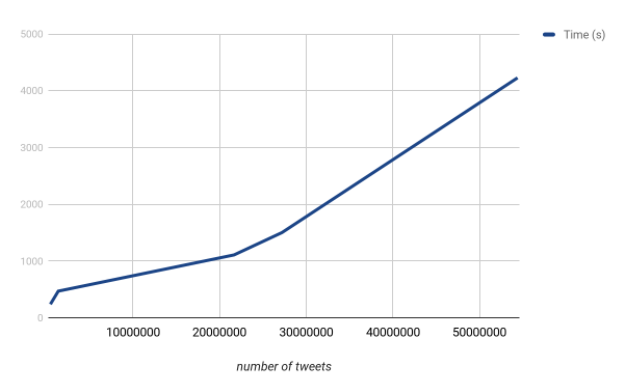
\includegraphics[width=.5\textwidth]{Figures/wordcountplot}
      \pdfnote{27M in 25 min}
       \begin{table}
      \centering
        \begin{tabular}{r r r}
        \hline
        \textbf{Number of tweets} & \textbf{Time (s)} & \textbf{Tweets/sec}\\
        \hline
        490199 & 238 & 2060 \\
        \hline
        1400884 & 469 & 2987 \\
        \hline
        21680851 & 1107 & 19585 \\
        \hline
        27199614 & 1500 & 18133 \\
        \hline
        54395957 & 4228 & 12866 \\
        \hline
        \end{tabular}
      \end{table}

    \end{center}
\end{frame}







\section{Future work}
\begin{frame}{Future work}
\begin{wideitemize}
  \item Improve resource specification (CPU, memory)
  \item Better Cassandra structure
  \item Unified authentification
  \item Extend the system with new features
\end{wideitemize}
\end{frame}





\hugeframe{Questions?}


\hugeframedouble{Thank you!}{
\begin{description}
  \addtolength{\itemsep}{5pt}
  \item[\textbf{Twitter}]  \href{http://twitter.com/casassaez}{@casassaez}
  \item[\textbf{Website}]  \href{http://gerard.space}{gerard.space}
  \item[\textbf{Repo}] \href{http://github.com/casassg/thesis}{github.com/casassg/thesis}

\end{description} 

}

% Commands to include a figure:
%\begin{figure}
%\includegraphics[width=\textwidth]{your-figure's-file-name}
%\caption{\label{fig:your-figure}Caption goes here.}
%\end{figure}

% \begin{table}
% \centering
% \begin{tabular}{l|r}
% Item & Quantity \\\hline
% Widgets & 42 \\
% Gadgets & 13
% \end{tabular}
% \caption{\label{tab:widgets}An example table.}
% \end{table}

% \end{frame}


\end{document}
